%!TEX root=../GaugeCNNTheory.tex


\section{Toy model: reflection equivariant M{\"o}bius convolutions}
\label{sec:mobius_conv}

To make the theoretical considerations in the previous sections more tangible, we turn now to an example application.
While not being of immediate practical importance, $\GM$-convolutions on the M\"obius strip are a suitable toy model since its geometry and the involved representation theory are particularly simple.
Due to its non-orientability, reference frames can only be (smoothly) preferred up to reflections.
As expected, coordinate independent CNNs, applying reflection equivariant template functions, outperform a naive, coordinate dependent implementation.
They are furthermore shown to be equivariant under the action of the M\"obius strip's isometry group.

\etocsettocdepth{3}
\etocsettocstyle{}{} % from now on only local tocs
\localtableofcontents

The following Section~\ref{sec:mobius_geometry} discusses the geometry of the flat M\"obius strip.
Due to its twist, its structure group can not be reduced further than to the reflection group~$G=\Flip$, such that one needs to consider a $\Flip$-atlas of gauges as visualized in Fig.~\ref{fig:mobius_conv_gauges}.
The isometry group is given by rotations along the strip and induces $\Flip$-valued gauge transformations.
$\RM$-coordinate independent feature fields, some of which are introduced in Section~\ref{sec:mobius_representations}, necessarily have to transform according to some representation of the reflection group.
Section~\ref{sec:mobius_cnn_ops_analytical} discusses orientation independent convolutional network operations.
This clarifies in particular the concept of $G$-steerable kernels but also covers reflection equivariant biases and nonlinearities.
A numerical implementation of the proposed model family is discussed and evaluated in Section~\ref{sec:mobius_experiment_main}.
The code is publicly available at \url{https://github.com/mauriceweiler/MobiusCNNs}.






\subsection{Geometry of the M\"obius strip}
\label{sec:mobius_geometry}

The manifold $M$ under consideration is the flat M\"obius strip with boundary as shown in Fig.~\ref{fig:weight_sharing_ambiguity} (right).
It~can be thought of as being constructed by taking a rectangular subset $[0,X] \times [0,Y]$ of $\R^2$ and gluing two opposing ends together in a twisted way.
Such defined, the M\"obius strip inherits the canonical metric of $\R^2$, which endows it with a Riemannian structure.
The metric specifies in particular a Levi-Civita connection and therefore exponential maps and parallel transporters, which are further discussed below.

\begin{figure}
    \centering
    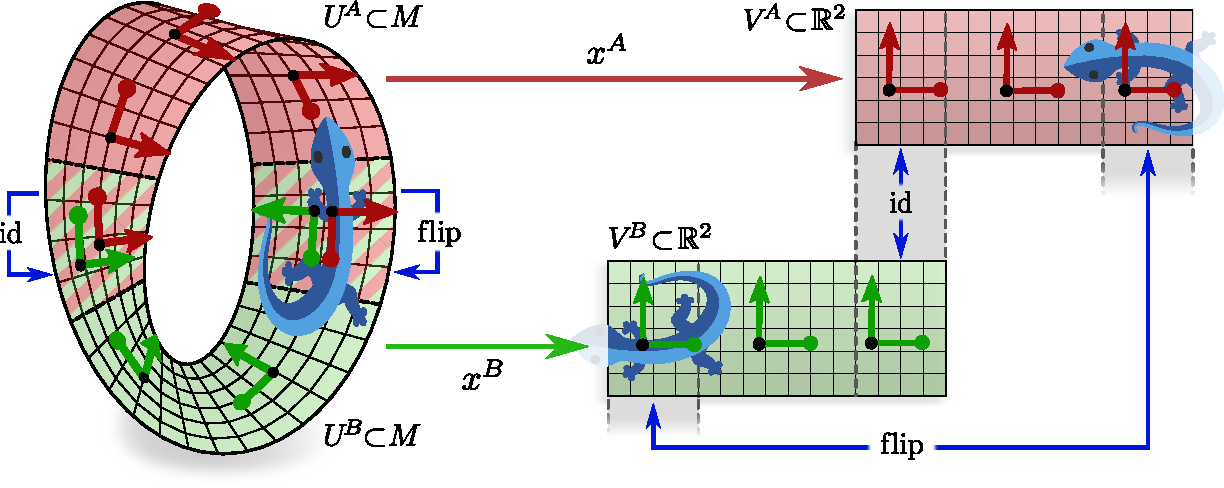
\includegraphics[width=\columnwidth]{figures/mobius_conv_gauges.pdf}
    \vspace*{.5ex}
    \caption{\small
        The flat geometry of the M\"obius strip allows for local subsets which can be isometrically identified with corresponding subsets of~$\R^2$.
        We fix an isometric atlas, consisting of two charts $x^A$ and $x^B$ on $U^A$ (red) and $U^B$ (green), which cover the whole strip.
        Gauges $\psi_p^X = \hat{d}x_p^X: \TpM \to \R^d$ for $p\in U^A$ are induced as chart differentials.
        Due to the twist of the M\"obius strip, the transition functions $g_p^{BA}$ will at one of the overlapping regions be trivial, while the other region will necessarily transition between gauges via flips~$s$.
        The chosen atlas of charts therefore induces an $\Flip$-atlas of gauges and implies a corresponding $\Flip$-structure $\RM$, consisting of two reflected frames at each point of~$M$.
        Each of the charts $x^X$ induces a smooth local frame field, given by the coordinate bases
        $\Big[\frac{\partial}{\partial x_i^X} \mkern-1mu\big|_p \Big] \raisebox{-2pt}{$\rule{0pt}{11pt}_{i=1}^d$}$.
        The flip in the transition functions at one overlap shows in a reflection of frames.
        {
        \\ \color{gray} \scriptsize
            (Lizards adapted under the Creative Commons Attribution 4.0 International
            \href{https://github.com/twitter/twemoji/blob/gh-pages/LICENSE-GRAPHICS}{\underline{license}}
            by courtesy of Twitter.)
        }
    }
    \label{fig:mobius_conv_gauges}
\end{figure}

A first question to answer when constructing a coordinate independent CNN is to which extent the choice of reference frames is ambiguous.
Given the Riemannian metric on the strip, we can restrict our attention to orthonormal frames.
One can furthermore single out one of the two directions \emph{along} the strip to (smoothly) disambiguate the rotation of the reference frames by aligning their first axes with this direction.
This leaves us with an ambiguity of frame handedness, with the two orientations corresponding to the two possible directions of the second frame axis perpendicular to the strip.
Being a non-orientable manifold, the M\"obius strip does not admit a globally smooth (or even continuous) choice of frame orientations.
To get an intuition about this statement, consider the attempt of constructing a smooth frame field by picking an arbitrary frame at a random position and to smoothly extend this choice over the whole strip.
After one revolution around the strip the constructed frames will unavoidably be reflected w.r.t. the initial frames, and therefore contradict the desired smoothness.
It is thus topologically \emph{impossible} to define an $\{e\}$-structure, i.e. a globally smooth field of frames, on the M\"obius strip.
We are thus left with an irreducible structure group
\begin{align}
    G \,=\, \Flip \,\cong\, \Z/2\Z \,,
\end{align}
which models the reflection of frames.
The reflection group contains only two elements, the identity $e$ and the reflection (Spiegelung) $s$, which are composed according to the following simple multiplication table:
\begin{align}\label{eq:reflection_multiplication_table}
\begin{tabular}{c|c@{\hspace{8pt}}c}
        & $e$ & $s$ \\ \hline
    $e$ & $e$ & $s$ \\
    $s$ & $s$ & $e$
\end{tabular}
\end{align}
The only nontrivial statement in this table is that two reflections annihilate, that is, $s^2=e$, or, equivalently, $s^{-1}=s$.
Given the irreducibility of the structure group $\Flip$, we will in the following need to consider the corresponding $\Flip$-structure $\RM$ which consists of two frames of opposing handedness at each point on the M\"obius strip.


To encode smooth $\RM$-coordinate independent feature fields on $M$, one needs to specify an $\Flip$-atlas, consisting of $\Flip$-related gauges that cover the whole strip.
We choose to do this by fixing an atlas of \emph{charts}
\begin{align}
    x^X: U^X \to V^X \subset \R^2
\end{align}
which cover the strip, and subsequently induce the gauges from it.
Fig.~\ref{fig:mobius_conv_gauges} visualizes such an atlas, consisting of two charts $x^A$ and $x^B$ on $U^A$ (red) and $U^B$ (green) which map two overlapping halves of the strip isometrically to corresponding rectangular regions of $\R^2$.
As described in Appendix~\ref{apx:chart_induced_bases_main}, the charts induce gauges, which are given by the chart differentials, that is,
\begin{align}
    \psi_p^X \,:=\, \hat{d}x^X_p :\ \TpM \to \R^2 \ \ \ \textup{for any}\,\ p\in U^X\,\ \text{and}\,\ X=A,B \,.
\end{align}
The transition functions coincide then with the Jacobians
$g^{BA} = \frac{\partial x^B}{\partial x^A}$.
Due to the twist, the transition maps are at one of the two overlapping regions all trivial, that is, $g_p^{BA} = e$, and on the other end necessarily reflected, i.e. $g_p^{BA} = s$.
The induced atlas of gauges is therefore indeed identified as an $\Flip$-atlas.
Being derived from coordinate charts, the smooth local frame fields corresponding to the gauges are just the usual coordinate bases, that is, the frames $\big[e_i^X \big]_{i=1}^d$ at $p\in U^X$ are given by
$\pig[\frac{\partial}{\partial x_i^X} \mkern-1mu\big|_p \pig] \raisebox{-2pt}{$\rule{0pt}{11pt}_{i=1}^d$}$.
Since the charts are isometric, the induced frame field is automatically orthonormal.
However, the two rectangular regions $V^A$ and $V^B$ in $\R^2$ must not be rotated relative to each other in order to induce an $\Flip$-atlas and a corresponding $\Flip$-structure~$\RM$.

We need to emphasize that the approach of inducing gauges via coordinate charts is not strictly necessary
-- it is just a convenient option since the \emph{flat} M\"obius strip is locally identified with regions of $\R^2$ in an \emph{isometric} way.
This will later allow us to transfer regular sampling grids from $\R^2$, like for instance the pixel grid $\Z^2$, to regular sampling grids on the strip.
As this is not possible for manifolds that are not locally flat, for instance meshes in computer graphics, most implementations on general manifolds (or meshes) assign coordinates immediately to the tangent spaces; see Section~\ref{sec:instantiations_mesh}.


The canonical Levi-Civita connection on the M\"obius strip defines a notion of parallel transport of tangent vectors.
Since the strip is locally isometric to the plane $\R^2$, this transport can on local patches be understood as flattening these patches out into a plane and moving the vectors as usual on~$\R^2$.
If no single patch can cover a path~$\gamma$, there will be an open covering such that the full transport is explained by a sequence of transporters over the local patches.
It is easy to see that the transport will relative to frames of the chosen $\Flip$-structure take values $g_\gamma^{A\widetilde{A}}$ in the reflection group $\Flip$.
This means that the Levi-Civita connection is $\Flip$-compatible with~$\RM$.
It does therefore imply well defined transporters $\rho\big( g_\gamma^{A\widetilde{A}} \big)$ of $\Flip$-associated feature vectors.


The group $\IsomRM$ of isometries that preserve the $\Flip$-structure contains all rotations which shift the strip along itself.
Note that a rotation once around the strip, which we denote by an angle of $2\pi$, does \emph{not} correspond to the identity but rather maps the strip in a reflected way on itself.
Only a rotation by $4\pi$, i.e. two full revolutions, map the strip back to itself.%
\footnote{
    The M\"obius strip is therefore seen to have the cylinder as double cover.
}
The action of the isometry group on the manifold and on reference frames is visualized in Fig.~\ref{fig:mobius_conv_isometries}.
Relative to coordinates, the isometry action will induce $\Flip$-valued gauge transformations.


\begin{figure}
    \centering
    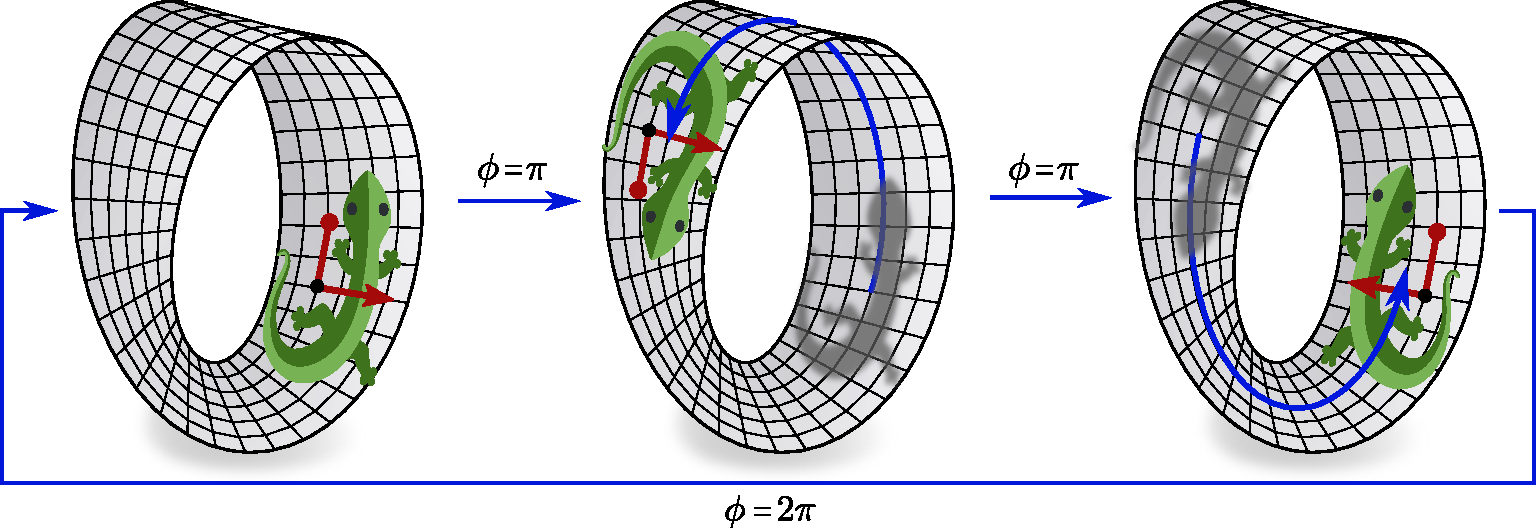
\includegraphics[width=\columnwidth]{figures/mobius_conv_isom.pdf}
    \caption{\small
        Visualization of the group of $\Flip$-structure preserving isometries $\IsomRM$ of the M\"obius strip, which is isomorphic to~$\SO2$.
        It consists of all rotations along the strip.
        Due to the twist, a rotation by $2\pi$, i.e. once around the strip, does not yet map it back to itself but results in a reflection.
        After a second revolution, that is, a total rotation of $4\pi$, the strip is mapped back to itself.
        Induced gauge transformations take values in $\Flip$.
        {
        \\ \color{gray} \scriptsize
            (Lizards adapted under the Creative Commons Attribution 4.0 International
            \href{https://github.com/twitter/twemoji/blob/gh-pages/LICENSE-GRAPHICS}{\underline{license}}
            by courtesy of Twitter.)
        }
    }
    \label{fig:mobius_conv_isometries}
\end{figure}








\subsection{Orientation independent feature fields}
\label{sec:mobius_representations}

The principle of covariance requires the feature fields on the M\"obius strip to be $\RM$-coordinate independent, that is, they need to be equivalently expressible relative to frames of either handedness.
They are therefore characterized by a choice of group representation $\rho: \Flip \to \GL{c}$ of the reflection group, which specifies the transformation of numerical feature vectors when switching between the two orientations.
We will in the following discuss a few possible choices of such field types.
The reader might want to check that the proposed representations are indeed group homomorphisms, satisfying $\rho(gh) = \rho(g)\rho(h)\,\ \forall\, g,h\in \Flip$, as demanded in Section~\ref{sec:feature_fields} and footnote~\ref{footnote:repr_group_homomorphism}.

The most basic example, which exists for any structure group, is the \emph{trivial representation}
\begin{align}
    \rhotriv: \Flip \to \GL{1}\ , \qquad 
    \begin{aligned}
        e &\mapsto \big[\mkern2mu 1 \mkern2mu\big] \\[2pt]
        s &\mapsto \big[\mkern2mu 1 \mkern2mu\big] \\
    \end{aligned}
    \quad ,
\end{align}
which assigns the ${1\!\times\!1}$ identity matrix to both group elements.
It models scalar fields $f_{\textup{triv}}$, which consist of one-dimensional feature vectors whose coordinatizations $f^A_{\textup{triv}}(p) \in \R^1$ stay \emph{invariant under frame reflections}.
A second one-dimensional representation is the \emph{sign-flip representation}
\begin{align}
    \rhosign: \Flip \to \GL{1}\ , \qquad 
    \begin{aligned}
        e &\mapsto \big[\mkern2mu 1 \mkern2mu\big] \\[2pt]
        s &\mapsto \big[\! \shortminus\!1 \big]
    \end{aligned}
    \quad .
\end{align}
It assigns the negative ${1\!\times\!1}$ identity matrix to reflections, and therefore describes pseudoscalar fields, i.e. one-dimensional feature fields $f_{\textup{sign}}$, whose numerical coefficients $f^A_{\textup{sign}}(p) \in \R^1$ \emph{change their sign under reflections}, \mbox{that is,} ${\rhosign(s)\cdot f^A_{\textup{sign}}(p) = -f^A_{\textup{sign}}(p)}$.
Since the trivial representation and the sign-flip representation are one-dimensional, they are both irreducible representations (irreps) of the reflection group.
In fact, they are the only two irreps of the reflection group.%
\footnote{
    The reflection group is isomorphic to the cyclic group $\Z/2\Z$ of order two.
    It is well known that the irreps of cyclic groups of order $N$ correspond to the $N$-th roots of unity, which are for $N=2$ just $+1$ (trivial) and $-1$ (sign-flip).
}

Since $\Flip$ is a finite group, it has a finite-dimensional (two-dimensional) \emph{regular representation}
\begin{align}
    \rhoreg: \Flip \to \GL{2}\ , \qquad 
    \begin{aligned}
        e &\mapsto
            \begin{bmatrix} \hspace{1.5pt}
                1 &\mkern-4mu 0 \hspace*{1.5pt} \\ \hspace{1.5pt} 0 &\mkern-4mu 1 \hspace*{1.5pt}
            \end{bmatrix} \\[2pt]
        s &\mapsto 
            \begin{bmatrix} \hspace{1.5pt}
                0 &\mkern-4mu 1 \hspace*{1.5pt} \\ \hspace{1.5pt} 1 &\mkern-4mu 0 \hspace*{1.5pt}
            \end{bmatrix}
    \end{aligned}
    \quad ,
\end{align}
which represents the group elements by permutation matrices.
By definition, the regular representation models the permutation of the group elements in $\Flip$ when acting on themselves.
Compare this to the columns of the multiplication table in Eq.~\eqref{eq:reflection_multiplication_table}:
the middle column can be thought of as originating from the action of $\rhoreg(e)$ on the leftmost column, while the swapped group elements in the right column correspond to the permutation described by the action of $\rhoreg(s)$ on the left column.
The regular feature fields $f_{\textup{reg}}$ of $\Flip$ are numerically represented by two-dimensional feature vectors $f^A_{\textup{reg}}(p) \in \R^2$ whose two \emph{channels are swapped under reflections}, that is,
$
    \rhoreg(s) \mkern-1mu\cdot\mkern-2mu f^A_{\textup{reg}}(p)
    \,=\,
    \begin{bmatrix} \hspace{1.5pt} 0 &\mkern-4mu 1 \hspace*{1.5pt} \\ \hspace{1.5pt} 1 &\mkern-4mu 0 \hspace*{1.5pt} \end{bmatrix}
    \mkern-4mu \cdot\mkern-4mu 
    \begin{bmatrix} f^A_{\textup{reg},1} \\ f^A_{\textup{reg},2} \end{bmatrix} \!(p)
    \,=\,
    \begin{bmatrix} f^A_{\textup{reg},2} \\ f^A_{\textup{reg},1} \end{bmatrix} \!(p)
$.


The regular representation is reducible, that is, it contains two proper invariant subspaces, which correspond in this case to the trivial and the sign-flip representation.
It can therefore equivalently be thought of as being constructed of the direct sum $\rhotriv \oplus \rhosign$ of those two irreps and a change of basis $Q$\,:
\begin{align}\label{eq:rho_reg_decomposition}
    \rhoreg(g)\ =\ Q\, \big( \rhotriv \!\oplus\mkern-1mu \rhosign \big)\mkern-2mu(g)\; Q^\top
    \quad\ \textup{where } \quad
    Q = \frac{1}{\sqrt{2}}
    \begin{bmatrix} \hspace{1.5pt}
        1 &\mkern-7mu \shortminus1 \hspace*{1.5pt} \\ \hspace{1.5pt} 1 &\mkern-7mu \phantom{\shortminus}1 \hspace*{1.5pt}
    \end{bmatrix}
\end{align}
The validity of this statement is easily asserted by inserting the r.h.s. for both group elements:
\begin{align}
    Q\, \big( \rhotriv \!\oplus\mkern-1mu \rhosign \big)\mkern-2mu(e)\; Q^\top
    \ =\ \frac{1}{2}
    \begin{bmatrix} \hspace{1.5pt}
        1 &\mkern-7mu \shortminus1 \hspace*{1.5pt} \\ \hspace{1.5pt} 1 &\mkern-7mu \phantom{\shortminus}1 \hspace*{1.5pt}
    \end{bmatrix} \mkern-6mu \cdot\mkern-6mu
    \begin{bmatrix} \hspace{1.5pt}
        1 &\mkern-7mu 0 \hspace*{1.5pt} \\ \hspace{1.5pt} 0 &\mkern-7mu 1 \hspace*{1.5pt}
    \end{bmatrix} \mkern-6mu \cdot\mkern-6mu
    \begin{bmatrix} \hspace{1.5pt}
        \phantom{\shortminus}1 &\mkern-7mu 1 \hspace*{1.5pt} \\ \hspace{1.5pt} \shortminus1 &\mkern-7mu 1 \hspace*{1.5pt}
    \end{bmatrix}
    \ =\ 
    \begin{bmatrix} \hspace{1.5pt}
        1 &\mkern-7mu 0 \hspace*{1.5pt} \\ \hspace{1.5pt} 0 &\mkern-7mu 1 \hspace*{1.5pt}
    \end{bmatrix}
    \ =\ \rhoreg(e)
\end{align}
\begin{align}
    Q\, \big( \rhotriv \!\oplus\mkern-1mu \rhosign \big)\mkern-2mu(s)\; Q^\top
    \,=\, \frac{1}{2}
    \begin{bmatrix} \hspace{1.5pt}
        1 &\mkern-7mu \shortminus1 \hspace*{1.5pt} \\ \hspace{1.5pt} 1 &\mkern-7mu \phantom{\shortminus}1 \hspace*{1.5pt}
    \end{bmatrix} \mkern-6mu \cdot\mkern-6mu
    \begin{bmatrix} \hspace{1.5pt}
        1 &\mkern-7mu \phantom{\shortminus}0 \hspace*{1.5pt} \\ \hspace{1.5pt} 0 &\mkern-7mu \shortminus1 \hspace*{1.5pt}
    \end{bmatrix} \mkern-6mu \cdot\mkern-6mu
    \begin{bmatrix} \hspace{1.5pt}
        \phantom{\shortminus}1 &\mkern-7mu 1 \hspace*{1.5pt} \\ \hspace{1.5pt} \shortminus1 &\mkern-7mu 1 \hspace*{1.5pt}
    \end{bmatrix}
    \,=\, \frac{1}{2}
    \begin{bmatrix} \hspace{1.5pt}
        1 &\mkern-7mu \phantom{\shortminus}1 \hspace*{1.5pt} \\ \hspace{1.5pt} 1 &\mkern-7mu \shortminus1 \hspace*{1.5pt}
    \end{bmatrix} \mkern-6mu \cdot\mkern-6mu
    \begin{bmatrix} \hspace{1.5pt}
        \phantom{\shortminus}1 &\mkern-7mu 1 \hspace*{1.5pt} \\ \hspace{1.5pt} \shortminus1 &\mkern-7mu 1 \hspace*{1.5pt}
    \end{bmatrix}
    \,=\, 
    \begin{bmatrix} \hspace{1.5pt}
        0 &\mkern-7mu 1 \hspace*{1.5pt} \\ \hspace{1.5pt} 1 &\mkern-7mu 0 \hspace*{1.5pt}
    \end{bmatrix}
    \,=\, \rhoreg(s)
\end{align}
More generally, any finite-dimensional representations of compact (including finite) groups is \emph{completely reducible} into a direct sum of irreps~\cite{gallier2019harmonicRepr,din2017reprLectureNotes,serre1977linear}.
This suggests that any covariant feature vector, transforming under a compact structure group, can up to a change of basis be constructed from irrep features.
As argued in~\cite{Weiler2019_E2CNN}, it is in this case indeed possible to reduce any \emph{linear} network operation to equivalent operations between irrep fields, which simplifies the construction of the space of $G$-steerable kernels in Eq.~\eqref{eq:G-steerable_kernel_space} and of invariant biases in Eq.~\eqref{eq:gauge_bias_solution_space}.
However, as we will see below, the specific choice of basis of equivalent field types has a quite significant impact on the model performance.
The reason for this is that \emph{nonlinear} network operations are sensitive to the chosen basis, i.e. to a specific choice from equivalent field types.













\subsection{Orientation independent convolutional networks}
\label{sec:mobius_cnn_ops_analytical}

In order to construct orientation independent CNNs on the M\"obius strip we need to instantiate the gauge equivariant layers from Section~\ref{sec:gauge_CNNs_local} for the reflection group~$\Flip$.
More specifically, each of the shared equivariant template functions defining the orientation independent layers needs to be instantiated for any choice of the considered field types $\rhotriv$, $\rhosign$ and $\rhoreg$.
The following Section~\ref{sec:mobius_bias} starts by solving for the spaces $\mathscr{B}^R_\rho$ of gauge invariant bias templates from Eq.~\eqref{eq:gauge_bias_solution_space}
Some admissible choices of gauge equivariant nonlinearities for the different field types are proposed in Section~\ref{sec:mobius_nonlin}.
Section~\ref{sec:mobius_kernel_spaces} will then derive the spaces $\KR$ of $\Flip$-steerable kernels (Eq.~\eqref{eq:G-steerable_kernel_space}) for each possible pair of input and output irreps.
While this section will mainly consist of theoretical derivations, the following Section~\ref{sec:mobius_experiment_main} will cover more practical implementation details.




\subsubsection{Orientation independent bias summation}
\label{sec:mobius_bias}

The space of biases templates that can be summed to a field of type $\rho$ without interfering with the coordinate independence assumption was in Section~\ref{sec:gauge_bias_summation} shown to be given by
\begin{align}
    \mathscr{B}^{\Flip}_\rho\ :=\ \big\{ b \in\R^c \;\big|\; b = \rho(g)\mkern2mu b\ \ \ \forall g\in \Flip \big\} \,.
\end{align}
For the case of the reflection group, there are only two group elements and thus two constraints.
The constraint for the identity element $g=e$ is trivially satisfied since $\rho(e) = \id_{\R^c}$ is by definition always the identity on~$\R^c$.
In the following it is therefore sufficient to restrict attention to the constraint $b = \rho(s)\mkern2mu b$ coming from the reflection $g=s$.

We start with the case of scalar fields, i.e. the trivial representation.
The reflection constraint then reads $b = \rhotriv(s)\mkern2mu b = b$, which is always satisfied.
It follows that the space of bias templates
\begin{align}
    \mathscr{B}^{\Flip}_{\scalebox{.8}{$\rho_{{\textup{triv}}}$}} = \R
\end{align}
remains unconstrained such that arbitrary real-valued biases can be summed to scalar fields.
For the sign-flip representation the reflection constraint becomes $b = \rhotriv(s)\, b = -b$ and is therefore only satisfied for biases which are zero:
\begin{align}
    \mathscr{B}^{\Flip}_{\scalebox{.8}{$\rho_{{\textup{sign}}}$}} = \{0\}
\end{align}
It is thus impossible to sum biases to sign-flip fields while maintaining coordinate independence.
Our third exemplary field type is the two-dimensional regular representation.
The corresponding reflectional constraint on $b\in\R^2$ reads
\begin{align}
    \begin{bmatrix} b_1 \\ b_2 \end{bmatrix}
    \ =\ 
    b
    \ =\ 
    \rhoreg(s)\mkern2mu b
    \ =\ 
    \begin{bmatrix} \hspace{1.5pt}
        0 &\mkern-7mu 1 \hspace*{1.5pt} \\ \hspace{1.5pt} 1 &\mkern-7mu 0 \hspace*{1.5pt}
    \end{bmatrix}
    \!\cdot\! \begin{bmatrix} b_1 \\ b_2 \end{bmatrix}
    \ =\ 
    \begin{bmatrix} b_2 \\ b_1 \end{bmatrix}
\end{align}
and leads to the one-dimensional solution space
\begin{align}\label{eq:bias_solution_space_regular}
    \mathscr{B}^{\Flip}_{\scalebox{.8}{$\rho_{{\textup{reg}}}$}} = 
    \big\{ b\in\R^2 \,\big|\, b_1=b_2 \big\} =
    \bigg\{ \begin{bmatrix} \beta \\ \beta \end{bmatrix} \,\bigg|\, \beta\in\R \bigg\} \ .
\end{align}
The coordinate independence of this constraint is intuitively clear:
since the regular representation swaps the two channels which make up the field, the bias summation is only then coordinate independent when the values summed to both channels are equal, such that their order does not matter.

As already claimed in Section~\ref{sec:gauge_bias_summation}, the solution space $\mathscr{B}^{\Flip}_\rho$ for a representation $\rho$ coincides exactly with its trivial subrepresentations.
This is certainly true for the trivial representation, to which one can sum any bias, and the sign-flip representation, which has itself no trivial subrepresentation and therefore does not admit biases at all.
A more interesting example is the regular representation, which was in Eq.~\ref{eq:rho_reg_decomposition} shown to decompose into a direct sum of the trivial and the sign-flip representation.
The one-dimensional solution space in Eq.~\ref{eq:bias_solution_space_regular} corresponds exactly to the single trivial subrepresentation contained in~$\rhoreg$.
To check the validity of this statement, note that the admissible biases for the direct sum representation $\rhotriv \oplus \rhosign$ are of the form $(\beta,\mkern1mu 0\mkern1mu)^\top$, where $\beta\in\R$.
This results can via the change of basis $Q$ be translated back to the regular representation, which indeed recovers our solution in Eq.~\eqref{eq:bias_solution_space_regular}:
\begin{align}
    Q \cdot\mkern-2mu \begin{bmatrix} \beta \\ 0 \end{bmatrix}
    \ \propto\ 
    \begin{bmatrix} \hspace{1.5pt}
        1 &\mkern-7mu \shortminus1 \hspace*{1.5pt} \\ \hspace{1.5pt} 1 &\mkern-7mu \phantom{\shortminus}1 \hspace*{1.5pt}
    \end{bmatrix}
    \!\cdot\! \begin{bmatrix} \beta \\ 0 \end{bmatrix}
    \ =\ 
    \begin{bmatrix} \beta \\ \beta \end{bmatrix}
\end{align}





\subsubsection{Orientation independent nonlinearities}
\label{sec:mobius_nonlin}

To construct a deep network, we need to come up with equivariant nonlinearities for each of the field types.
As already discussed in Section~\ref{sec:gauge_nonlinearities}, scalar fields can due to their invariance under gauge transformations be acted on by any nonlinearity $\mathscr{s}_{\textup{triv}}: \R\to\R$.
Usual choices are the pointwise ReLU or ELU nonlinearities.
For the sign-flip fields one might take the absolute value $\lVert f^A_{\textup{sign}}(p) \rVert$ of feature vectors, which maps the sign-flip field to a scalar field.
In our implementation below we instead use nonlinearities of the form
\begin{align}\label{eq:signflip_nonlin}
    \mathscr{s}_{\textup{sign}}: \mathscr{f} \ \mapsto\ 
    \operatorname{ReLU} \!\big( \lVert \mathscr{f} \rVert - b \big) \mkern-2mu\cdot\!
    \frac{\mathscr{f}}{\lVert \mathscr{f} \rVert},
\end{align}
where $b\in\R^+$ is a learnable bias parameter.
This choice is easily seen to map sign-flip fields to sign-flip fields since the first multiplicand is acting on the gauge invariant norm of feature vectors while the second multiplicand is preserving the feature vector's sign.
As a permutation representation, the regular representation allows for any pointwise nonlinearity, for instance ReLUs, to act on the individual field channels without changing the field type:
\begin{align}
    \rhoreg(s) \circ \mathscr{s}_{\textup{reg}} \begin{bmatrix} \mathscr{f}_1 \\ \mathscr{f}_2 \end{bmatrix}
    \ =\ 
    \begin{bmatrix} \hspace{1.5pt}
        0 &\mkern-7mu 1 \hspace*{1.5pt} \\ \hspace{1.5pt} 1 &\mkern-7mu 0 \hspace*{1.5pt}
    \end{bmatrix}
    \begin{bmatrix} \operatorname{ReLU}(\mathscr{f}_1) \\ \operatorname{ReLU}(\mathscr{f}_2) \end{bmatrix}
    \ =\ 
    \begin{bmatrix} \operatorname{ReLU}(\mathscr{f}_2) \\ \operatorname{ReLU}(\mathscr{f}_1) \end{bmatrix}
    \ =\ 
    \mathscr{s}_{\textup{reg}} \begin{bmatrix} \mathscr{f}_2 \\ \mathscr{f}_1 \end{bmatrix}
    \ =\ 
    \mathscr{s}_{\textup{reg}} \circ \rhoreg(s) \begin{bmatrix} \mathscr{f}_1 \\ \mathscr{f}_2 \end{bmatrix}
\end{align}
While the regular representation is linearly equivalent to $\rhotriv\oplus\rhosign$, we can not apply independent pointwise nonlinearities on the two channels in the irrep basis.
This substantiates the claim that nonlinearities make the networks sensitive to the particular choice of basis of the representation.








\subsubsection{Orientation independent convolutions}
\label{sec:mobius_kernel_spaces}

The last operations that we instantiate here are reflection equivariant convolutions.
This requires us on the one hand to explain the exponential map and parallel transport on the strip, and on the other hand to solve for the $\Flip$-steerable kernel spaces.
Due to the flat geometry of $M$ and the use of isometric charts, the former is almost trivial:
features are transported similarly as on $\R^2$, with the only difference that the feature vectors might experience a reflection by~$\rho(s)$.
Our implementation of this part is visualized in Fig.~\ref{fig:mobius_conv_numerical}, which is further explained in the following Section~\ref{sec:mobius_implementation}.
The current section focuses exclusively on the analytical solution of the kernel spaces.

For the M\"obius strip with $\Flip$-structure, the space of $\Flip$-steerable kernels from Eq.~\eqref{eq:G-steerable_kernel_space} is given by
\begin{align}
    \KR :=\ \Big\{ K\!: \R^2 \to \R^{\cout\times\cin} \,\Big|\,
    K(g\mkern1mu\mathscr{v}) = \rhoout(g) \mkern-2mu\cdot\mkern-2mu K(\mathscr{v}) \mkern-2mu\cdot\mkern-2mu \rhoin(g) \quad \forall\ \mathscr{v} \in \R^2,\,\ g\in \Flip \Big\} \,,
\end{align}
where we dropped the determinant factor $\detg=1$ and removed all inverses since ${g^{-1} \!=\! g\ \ \ \forall\mkern4mu g \in \Flip}$.
As~in the case of equivariant biases, the constraint coming from the identity element is trivially satisfied, such that only the reflectional constraint remains.
Reflection equivariant kernels are therefore characterized by the single constraint
\begin{align}
    K(s.\mathscr{v})\ =\ \rhoout(s) \mkern-1mu\cdot\mkern-1mu K(\mathscr{v}) \mkern-1mu\cdot\mkern-1mu \rhoin(s) \qquad \forall\: \mathscr{v} \in \R^2 \,,
\end{align}
which requires that the reflected kernel $K(s.\mathscr{v})$ equals the non-reflected kernel $K(\mathscr{v})$ after being acted on by the input and output field representation.
We will in the following solve this constraint for all nine pairs of field types.
The resulting kernels, all of which are in one or another sense symmetric under reflections, are visualized in Table~\ref{tab:reflection_steerable_kernels}.

\begin{SCtable}
    \hspace*{-5.ex}
    \def\figfolder{figures/kernels/}
    \def\figheight{0.08\columnwidth}
    \newlength{\vertSkip}
    \newlength{\eqToKernelSkip}
    \setlength\vertSkip{4.5ex}
    \setlength\eqToKernelSkip{1.5ex}
    \newcommand\cellTstrut{\rule{0pt}{3.5ex}}
    \footnotesize
    \setlength{\tabcolsep}{4pt}
    \begin{tabular}{r|c|c|c}
        \diagbox[height=18pt]{\raisebox{3pt}{$\rhoout$}}{\raisebox{-0pt}{$\rhoin$}}
        & trivial & sign-flip & regular \\
        \hline
        \cellTstrut
        %%%%%%%%%%%%%% FIRST ROW %%%%%%%%%%%%%%%
        \multirow{2}{*}{
            \hspace*{-1.5ex}
            trivial
            \hspace*{-1ex}
            \rule{0pt}{5.5ex}
            }
        & $\Koo(s.\mathscr{v}) = \Koo(\mathscr{v})$
        & $\Koo(s.\mathscr{v}) = \minus\Koo(\mathscr{v})$
        & $\Koo(s.\mathscr{v}) = \Kot(\mathscr{v})$
        \\[\eqToKernelSkip]
        & $\begin{pmatrix} \includegraphicstotab[height=\figheight]{\figfolder K_symmetric.png} \end{pmatrix}$
        & $\begin{pmatrix} \includegraphicstotab[height=\figheight]{\figfolder K_antisymmetric.png} \end{pmatrix}$
        & $\begin{pmatrix}
            \includegraphicstotab[height=\figheight]{\figfolder K_crisp_1.png} \mkern4mu, & \mkern-16mu
            \includegraphicstotab[height=\figheight]{\figfolder K_crisp_1f.png}
          \end{pmatrix}$ 
        \hspace{-6pt}
        \\[\vertSkip]
        \hline
        \cellTstrut
        %%%%%%%%%%%%%% SECOND ROW %%%%%%%%%%%%%%%
        \multirow{2}{*}{
            \hspace*{-1.5ex}
            sign-flip
            \hspace*{-1ex}
            \rule{0pt}{5.5ex}
            }
        & $\Koo(s.\mathscr{v}) = \minus\Koo(\mathscr{v})$
        & $\Koo(s.\mathscr{v}) = \Koo(\mathscr{v})$
        & $\Koo(s.\mathscr{v}) = \minus\Kot(\mathscr{v})$
        \\[\eqToKernelSkip]
        & $\begin{pmatrix} \includegraphicstotab[height=\figheight]{\figfolder K_antisymmetric.png} \end{pmatrix} $
        & $\begin{pmatrix} \includegraphicstotab[height=\figheight]{\figfolder K_symmetric.png} \end{pmatrix} $
        & $\begin{pmatrix}
            \includegraphicstotab[height=\figheight]{\figfolder K_crisp_1.png} \mkern4mu, & \mkern-16mu
            \includegraphicstotab[height=\figheight]{\figfolder K_crisp_1f_inverted.png}
          \end{pmatrix} $ 
        \hspace{-6pt}
        \\[\vertSkip]
        \hline
        \rule{0pt}{5.ex}
        %%%%%%%%%%%%%% THIRD ROW %%%%%%%%%%%%%%%
        \multirow{2}{*}{
            \hspace*{-1.5ex}
            regular
            \hspace*{-1ex}
            \rule{0pt}{10.5ex}
            }
        & $\Koo(s.\mathscr{v}) = \Kto(\mathscr{v})$
        & $\Koo(s.\mathscr{v}) = \minus\Kto(\mathscr{v})$
        & \makecell{
            $\Koo(s.\mathscr{v}) = \Ktt(\mathscr{v})$ \\[.6ex]
            $\Kot(s.\mathscr{v}) = \Kto(\mathscr{v})$
          }
        \hspace{-6pt}
        \\[3.ex]
        & $\begin{pmatrix}
            \includegraphicstotab[height=\figheight]{\figfolder K_crisp_1.png} \\
            \includegraphicstotab[height=\figheight]{\figfolder K_crisp_1f.png}
          \end{pmatrix}$
        & $\begin{pmatrix}
            \includegraphicstotab[height=\figheight]{\figfolder K_crisp_1.png} \\
            \includegraphicstotab[height=\figheight]{\figfolder K_crisp_1f_inverted.png}
          \end{pmatrix}$
        & $\begin{pmatrix}
            \includegraphicstotab[height=\figheight]{\figfolder K_crisp_1.png} \mkern4mu, & \mkern-16mu
            \includegraphicstotab[height=\figheight]{\figfolder K_crisp_3.png} \\
            \includegraphicstotab[height=\figheight]{\figfolder K_crisp_3f.png} \mkern4mu, & \mkern-16mu
            \includegraphicstotab[height=\figheight]{\figfolder K_crisp_1f.png}
          \end{pmatrix}$
    \end{tabular}
    %%%%%%%%%%%%%%%%%%%%%%%%%%%%%%%%%%%%%%%%%%%%%%%%%%%%%%%%%%%%%%%%%%%%%%%%%%%%%%%%%%%%%%%%%%%%%%%%%%%%%%%
    \captionsetup{width=1.\textwidth}
    \caption[]{\small
        \protect\rule{0ex}{8ex} % vertical position
        Visualization of reflection-steerable kernels in $\KR$ for all considered pairs of input and output field types $\rhoin$ and $\rhoout$.
        In general, these kernels need to satisfy the $\Flip\mkern-1.2mu$-steerability kernel constraint $K(s.\mathscr{v})\ =\ \rhoout(s) \mkern-1mu\cdot\mkern-1mu K(\mathscr{v}) \mkern-1mu\cdot\mkern-1mu \rhoin(s)$ where $K: \R^2 \to \R^{\cout\times\cin}$.
        Each entry of the table states the specific constraint for the corresponding input and output representations and visualizes one exemplary steerable kernel.
        Note that the constraint binds the reflected kernel $K(s.\mathscr{v})$ to a linear transformation of the unreflected kernel $K(\mathscr{v})$ by the input and output representation.
        It results therefore in reflectional symmetries of the kernels.
    }
    \label{tab:reflection_steerable_kernels}
\end{SCtable}


\begin{itemize}
\setlength{\itemindent}{-2em}
\setlength{\itemsep}{.5em}
    \item[{\rule[2.0pt]{2pt}{2pt}}]
    \textbf{scalar $\bm\to$ scalar:}
        Kernels
        $K = \pig[\Koo\pig]: \R^2 \to \R^{1\times1}$
        which map between scalar fields are required to satisfy the constraint
        \begin{align}
                \pig[\Koo\pig] \mkern-1mu (s.\mathscr{v})
            \ =\ 
                \big[\mkern2mu 1 \mkern2mu\big]
                \!\cdot\!
                \pig[\Koo\pig] \mkern-1mu (\mathscr{v})
                \cdot\!
                \big[\mkern2mu 1 \mkern2mu\big]
            \ =\ 
                \pig[\Koo\pig] \mkern-1mu (\mathscr{v})
            \qquad \forall\ \mathscr{v} \in \R^2 \,.
        \end{align}
        They are necessarily \emph{symmetric} (invariant) under reflections; see the upper left entry in Table~\ref{tab:reflection_steerable_kernels}.
    \item[{\rule[2.0pt]{2pt}{2pt}}]
    \textbf{scalar $\bm\to$ sign-flip:}
        The kernels $K = \pig[\Koo\pig]: \R^2 \to \R^{1\times1}$ which map a scalar field to a sign-flip field need to satisfy
        \begin{align}
                \pig[\Koo\pig] \mkern-1mu (s.\mathscr{v})
            \ =\ 
                \big[\! \shortminus\!1 \big]
                \!\cdot\!
                \pig[\Koo\pig] \mkern-1mu (\mathscr{v})
                \cdot\!
                \big[\mkern2mu 1 \mkern2mu\big]
            \ =\
                -\pig[\Koo\pig] \mkern-1mu (\mathscr{v})
            \qquad \forall\ \mathscr{v} \in \R^2 \,.
        \end{align}
        This implies \emph{antisymmetric} kernels as visualized in the middle row in the first column of Table~\ref{tab:reflection_steerable_kernels}.
    \item[{\rule[2.0pt]{2pt}{2pt}}]
    \textbf{scalar $\bm\to$ regular:}
        In order to map from a scalar field to a regular feature field one needs to apply kernels of the form
        $K = \begin{bmatrix} \Koo \\ \Kto \end{bmatrix}: \R^2 \to \R^{2\times1}$,
        which map from one input channel to two output channels.
        The demanded permutation of the output channels is guaranteed if the kernel satisfies
        \begin{align}\label{eq:constraint_s2r}
                \begin{bmatrix} \Koo \\ \Kto \end{bmatrix} \mkern-4mu (s.\mathscr{v})
            \ =\ 
                \begin{bmatrix} \hspace{1.5pt} 0 &\mkern-4mu 1 \hspace*{1.5pt} \\ \hspace{1.5pt} 1 &\mkern-4mu 0 \hspace*{1.5pt} \end{bmatrix}
                \!\cdot\!
                \begin{bmatrix} \Koo \\ \Kto \end{bmatrix} \mkern-4mu (\mathscr{v})
                \cdot\!
                \big[\mkern2mu 1 \mkern2mu\big]
            \ =\ 
                \begin{bmatrix} \Kto \\ \Koo \end{bmatrix} \mkern-4mu (\mathscr{v})
            \qquad \forall\ \mathscr{v} \in \R^2 \,.
        \end{align}
        This constraint requires that the two channels contain kernels which are \emph{reflected copies} of each other, that is,
        $\Koo(s.\mathscr{v}) = \Kto(\mathscr{v})$ for all $\mathscr{v} \in \R^2$
        (this already covers the second line of the constraint in Eq.~\eqref{eq:constraint_s2r}).
        This case is visualized in the bottom left entry of Table~\ref{tab:reflection_steerable_kernels}.
    %%%%%%%%%%%%%%%%%%%%%%%%%%%%%%%%%%%%%%%%%%%%%%%%%%%%%%%%%%%%%%%%%%%%%%%%%%%%%%%%%%%%%%%%%%%%%%%%%%%%%%
    \item[{\rule[2.0pt]{2pt}{2pt}}]
    \textbf{sign-flip $\bm\to$ scalar:}
        Kernels
        $K = \pig[\Koo\pig]: \R^2 \to \R^{1\times1}$
        that map from sign-flip to scalar fields are again \emph{antisymmetric} since they need to satisfy the same constraint
        \begin{align}
                \pig[\Koo\pig] \mkern-1mu (s.\mathscr{v})
            \ =\ 
                \big[\mkern2mu 1 \mkern2mu\big]
                \!\cdot\!
                \pig[\Koo\pig] \mkern-1mu (\mathscr{v})
                \cdot\!
                \big[\! \shortminus\!1 \big]
            \ =\ 
                -\pig[\Koo\pig] \mkern-1mu (\mathscr{v})
            \qquad \forall\ \mathscr{v} \in \R^2
        \end{align}
        like kernels which map in the opposite direction.
    \item[{\rule[2.0pt]{2pt}{2pt}}]
    \textbf{sign-flip $\bm\to$ sign-flip:}
        The kernels
        $K = \pig[\Koo\pig]: \R^2 \to \R^{1\times1}$
        which preserve the transformation behavior of sign-flip fields are \emph{symmetric} since the two sign inversions in the constraint
        \begin{align}
                \pig[\Koo\pig] \mkern-1mu (s.\mathscr{v})
            \ =\ 
                \big[\! \shortminus\!1 \big]
                \!\cdot\!
                \pig[\Koo\pig] \mkern-1mu (\mathscr{v})
                \cdot\!
                \big[\! \shortminus\!1 \big]
            \ =\ 
                \pig[\Koo\pig] \mkern-1mu (\mathscr{v})
            \qquad \forall\ \mathscr{v} \in \R^2
        \end{align}
        cancel out.
    \item[{\rule[2.0pt]{2pt}{2pt}}]
    \textbf{sign-flip $\bm\to$ regular:}
        In the case of kernels
        $K = \begin{bmatrix} \Koo \\ \Kto \end{bmatrix}: \R^2 \to \R^{2\times1}$
        which map from sign-flip to regular feature fields, we get the constraint
        \begin{align}
                \begin{bmatrix} \Koo \\ \Kto \end{bmatrix} \mkern-4mu (s.\mathscr{v})
            \ =\ 
                \begin{bmatrix} \hspace{1.5pt} 0 &\mkern-4mu 1 \hspace*{1.5pt} \\ \hspace{1.5pt} 1 &\mkern-4mu 0 \hspace*{1.5pt} \end{bmatrix}
                \!\cdot\!
                \begin{bmatrix} \Koo \\ \Kto \end{bmatrix} \mkern-4mu (\mathscr{v})
                \cdot\!
                \big[\! \shortminus\!1 \big]
            \ =\ 
                - \begin{bmatrix} \Kto \\ \Koo \end{bmatrix} \mkern-4mu (\mathscr{v})
            \qquad \forall\ \mathscr{v} \in \R^2 \,.
        \end{align}
        The two lines imply each other, such that they can be summarized by the single kernel constraint
        ${\Koo(s.\mathscr{v}) = -\Kto(\mathscr{v})}\ \ \forall \mathscr{v}\in \R^2$.
        This constraint requires that the two channels of the kernel contain \emph{reflected, negated copies} of each other; see the visualization in the middle of the bottom row of Table~\ref{tab:reflection_steerable_kernels}.
    %%%%%%%%%%%%%%%%%%%%%%%%%%%%%%%%%%%%%%%%%%%%%%%%%%%%%%%%%%%%%%%%%%%%%%%%%%%%%%%%%%%%%%%%%%%%%%%%%%%%%%
    \item[{\rule[2.0pt]{2pt}{2pt}}]
    \textbf{regular $\bm\to$ scalar:}
        The kernels which map regular feature fields to scalar fields have two input channels and one output channel and are therefor of the form
        $K = \pig[\Koo \,,\, \Kot\pig]: \R^2 \to \R^{1\times2}$.
        The constraint
        \begin{align}
                \pig[\Koo \,,\, \Kot\pig] \mkern-1mu (s.\mathscr{v})
            \ =\ 
                \big[\mkern2mu 1 \mkern2mu\big]
                \!\cdot\!
                \pig[\Koo \,,\, \Kot\pig] \mkern-1mu (\mathscr{v})
                \cdot\!
                \begin{bmatrix} \hspace{1.5pt} 0 &\mkern-4mu 1 \hspace*{1.5pt} \\ \hspace{1.5pt} 1 &\mkern-4mu 0 \hspace*{1.5pt} \end{bmatrix}
            \ =\ 
                \pig[\Kot \,,\, \Koo\pig] \mkern-1mu (\mathscr{v})
            \qquad \forall\ \mathscr{v} \in \R^2 \,,
        \end{align}
        which can be reduced to the requirement
        $\Koo(s.\mathscr{v}) = \Kot(\mathscr{v})\ \ \forall \mathscr{v} \in \R^2$,
        again demands that the two entries of the kernel contain \emph{reflected copies} of each other.
    \item[{\rule[2.0pt]{2pt}{2pt}}]
    \textbf{regular $\bm\to$ sign-flip:}
        Mappings from regular feature fields to sign-flip fields utilize kernels
        $K = \pig[\Koo,\, \Kot\pig]: \R^2 \to \R^{1\times2}$
        that satisfy
        \begin{align}
                \pig[\Koo \,,\, \Kot\pig] \mkern-1mu (s.\mathscr{v})
            \ =\ 
                \big[\! \shortminus\!1 \big]
                \!\cdot\!
                \pig[\Koo \,,\, \Kot\pig] \mkern-1mu (\mathscr{v})
                \cdot\!
                \begin{bmatrix} \hspace{1.5pt} 0 &\mkern-4mu 1 \hspace*{1.5pt} \\ \hspace{1.5pt} 1 &\mkern-4mu 0 \hspace*{1.5pt} \end{bmatrix}
            \ =\ 
                - \pig[\Kot \,,\, \Koo\pig] \mkern-1mu (\mathscr{v})
            \qquad \forall\ \mathscr{v} \in \R^2 \,,
        \end{align}
        or, equivalently, $\Koo(s.\mathscr{v}) = -\Kot(\mathscr{v})\ \ \forall \mathscr{v} \in \R^2$.
        As probably already expected, they are made up from kernels whose two channels contain \emph{reflected, negated copies} of another.
    \item[{\rule[2.0pt]{2pt}{2pt}}]
    \textbf{regular $\bm\to$ regular:}
        Lastly, we need to consider kernels
        $K = \begin{bmatrix} \Koo &\mkern-12mu \Kot \\ \Kto &\mkern-12mu \Ktt \end{bmatrix}: \R^2 \to \R^{2\times2}$
        which map regular fields to regular fields and therefore have $2\times2$ matrices as codomain.
        Their constraint, coming from a left and right multiplication with the regular representation, becomes
        \begin{align}
                \begin{bmatrix} \Koo &\mkern-12mu \Kot \\ \Kto &\mkern-12mu \Ktt \end{bmatrix} \mkern-4mu (s.\mathscr{v})
            \ =\ 
                \begin{bmatrix} \hspace{1.5pt} 0 &\mkern-4mu 1 \hspace*{1.5pt} \\ \hspace{1.5pt} 1 &\mkern-4mu 0 \hspace*{1.5pt} \end{bmatrix}
                \!\cdot\!
                \begin{bmatrix} \Koo &\mkern-12mu \Kot \\ \Kto &\mkern-12mu \Ktt \end{bmatrix} \mkern-4mu (\mathscr{v})
                \cdot\!
                \begin{bmatrix} \hspace{1.5pt} 0 &\mkern-4mu 1 \hspace*{1.5pt} \\ \hspace{1.5pt} 1 &\mkern-4mu 0 \hspace*{1.5pt} \end{bmatrix}
            \ =\ 
                \begin{bmatrix} \Ktt &\mkern-12mu \Kto \\ \Kot &\mkern-12mu \Koo \end{bmatrix} \mkern-4mu (\mathscr{v})
            \qquad \forall\ \mathscr{v} \in \R^2 \,.
        \end{align}
        This is equivalent to the two independent constraints
        \begin{align}
            \Koo(s.\mathscr{v}) = \Ktt(\mathscr{v}) \quad \forall \mathscr{v} \in \R^2
        \end{align}
        and
        \begin{align}
            \Kot(s.\mathscr{v}) = \Kto(\mathscr{v}) \quad \forall \mathscr{v} \in \R^2 \,,
        \end{align}
        which couple the four kernel entries such that there are \emph{two pairs of mutually reflected kernels}.
        This case is visualized in the bottom right entry of Table~\ref{tab:reflection_steerable_kernels}.
\end{itemize}

While the derived results tell us how to map between individual feature fields, neural networks typically assume feature spaces that consist of multiple, potentially differing feature fields.
The kernels which map between these stacks of feature fields can be thought of as being built from blocks which map between the individual fields.
To give an example, consider the case where both the input and output feature spaces contain one of the discussed representations each, that is, $\rhoin = \rhoout = \rhotriv \oplus \rhosign \oplus \rhoreg$.
The number of input and output channels is then $\cin=\cout=1+1+2=4$, such that the full kernel is of the form $K: \R^2 \to \R^{4\times4}$.
Since the input and output representations are defined as direct sums, they are block diagonal.
The full constraint decouples thus into nine independent constraints between all pairs of individual input and output fields, which correspond in this case exactly to the nine solutions presented above.
The $4\times4$ entries of the full kernel will therefore be required to have the same symmetries as the $4\times4$ kernels which are visualized in Table~\ref{tab:reflection_steerable_kernels} as a whole.

For completeness, we briefly elaborate on general kernel field transforms and isometry equivariant kernel field transforms on the M\"obius strip.
In the general case the smooth kernel field remains entirely unrestricted, that is, no weights need to be shared and the individual kernels are not required to have any reflectional symmetries whatsoever.
In order for the kernel field transform to be equivariant w.r.t. isometries, the applied kernel field is required to be invariant under their action.
This requires weights to be shared over the isometry orbits, which come in two different types.
The first type corresponds to that single orbit which lies exactly in the middle of the strip.
Points on this orbit return back to themselves after one revolution around the strip, while the strip itself is reflected over this central orbit.
An $\IsomRM$-invariant kernel field will have some kernel shared over this central orbit, however, this kernel is required to have reflectional symmetries like the $\Flip$-steerable kernels in Table~\ref{tab:reflection_steerable_kernels}.
This is the case since the kernels are after one revolution mapped in a reflected way on themselves while the kernel field is required to be isometry invariant.%
\footnote{
    Section~\ref{sec:quotient_kernel_fields} describes such situations in a more general setting as \emph{stabilizer subgroup} constraints of the isometry group.
    In the current case, the subgroup of rotations once around the strip stabilizes the points on the central orbit.
    It is isomorphic to the reflection group and therefore leads to reflectional symmetries in the kernels.
}
Any other orbit is of the second orbit type.
Consider some point at a given distance from the central orbit.
The isometry action will move this point at this distance from the center along the strip.
However, it will not return to the initial point after one revolution but to that point which lies at the same distance on the opposite of the central orbit.
Only after a second revolution around the strip the orbit will close.
The demanded isometry invariance of the kernel field will thus require kernels to be shared over all points with the same distance in either direction of the strip's center (but allows for different kernels at different distances).
In contrast to the central orbit's kernel, these kernels are not required to be reflection equivariant themselves.
This analysis shows that any isometry equivariant kernel field transform requires $\Flip$-steerable kernels, although strictly only on the central orbit.
Conversely, the convolutional kernel field, corresponding to the application of the same $\Flip$-steerable kernels on the whole manifold, is certainly invariant under isometries.
The orientation independent convolution on the M\"obius strip is therefore $\IsomRM$-equivariant, which is empirically confirmed below.
















\subsection{Numerical implementation and evaluation of M\"obius convolutions}
\label{sec:mobius_experiment_main}

Being prepared with the analytical derivations in the previous sections we are ready to discuss a numerical implementation of orientation independent CNNs on the M\"obius strip.
After doing so in Section~\ref{sec:mobius_implementation}, we evaluate the models for different choices of field types and compare them with a naive, orientation dependent implementation in Section~\ref{sec:mobius_evaluation}.

The implementation is publicly available at \url{https://github.com/mauriceweiler/MobiusCNNs}.



\subsubsection{Numerical implementation}
\label{sec:mobius_implementation}

\paragraph{Feature spaces:}
The first question to answer when implementing convolutions on the M\"obius strip is how the feature fields should be represented numerically.
Since the M\"obius strip is a flat manifold, we can conveniently inherit (subsets of) the regular sampling grid $\Z^2$ from $\R^2$ over to the strip.
This intuition is formalized by the pullbacks
$f^X\circ \big(x^X\big)^{-1}: V^X \to \R^c$
of the local feature field coordinatizations
$f^X: U^X \to \R^c$
via the (inverse) charts
$\big(x^X\big)^{-1}: V^X \to U^X$
to a new domain $V^X \subset \R^2$,
where $X=A,B$.
The numerical discretization is then defined as a restriction
$f^X\circ \big(x^X\big)^{-1} \big|_{V^X\cap\mkern2mu\Z^2}$
of the pullback to the sampling grid, which is in Fig.~\ref{fig:mobius_conv_gauges} shown as an overlay.


\begin{figure}
    \begin{subfigure}[t!]{.6\linewidth}
        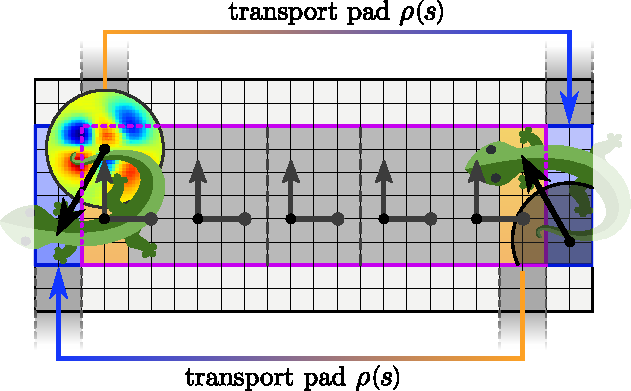
\includegraphics[width=\linewidth]{figures/mobius_conv_numerical.pdf}
    \end{subfigure}
    % new paragraph for correct alignment
    \par
    % (manually) wrapped caption, adapted from
    % https://tex.stackexchange.com/questions/158868/is-it-possible-to-let-captions-wrap-a-bit-around-includegraphics-within-figures
    % https://tex.stackexchange.com/questions/51839/wrap-caption-around-tikz-figure/51842#51842
    % The caption
    \vspace*{\dimexpr-\parskip-160.pt\relax}% Skip backwards over last left-aligned image
    \parshape 18 % Set flow of caption: N lines...
        .62\textwidth .37\textwidth % First N-1 start @ .62\textwidth with a width of .37\textwidth
        .62\textwidth .37\textwidth
        .62\textwidth .37\textwidth
        .62\textwidth .37\textwidth
        .62\textwidth .37\textwidth
        .62\textwidth .37\textwidth
        .62\textwidth .37\textwidth
        .62\textwidth .37\textwidth
        .62\textwidth .37\textwidth
        .62\textwidth .37\textwidth
        .62\textwidth .37\textwidth
        .62\textwidth .37\textwidth
        .62\textwidth .37\textwidth
        .62\textwidth .37\textwidth
        .62\textwidth .37\textwidth
        .62\textwidth .37\textwidth
        .62\textwidth .37\textwidth
        .01\textwidth .98\textwidth % the last (N-th) line flows from 0 to .99 = .62+.37 = .01+.98 ad infinitum
    \makeatletter
    \setcounter{\@captype}{\value{\@captype}-1} % \setcounter{CounterName}{number}
    \refstepcounter{\@captype}% Increase float/caption counter
    \addcontentsline{\csname ext@\@captype\endcsname}{\@captype}% Add content to "List of..."
        {\protect\numberline{\csname the\@captype\endcsname}{ToC entry}}%
    \small % switch to small font for caption and Figure XX:
    \csname fnum@\@captype\endcsname: % Float caption + #
    \makeatother
    % Actual caption
        Numerical representation of feature fields on the M\"obius strip and Levi-Civita transport of feature vectors during the convolution.
        The flat geometry of the strip allows to cut it open and flatten it out isometrically to the magenta rectangle.
        When assigning the canonical reference frames of~$\R^2$ this corresponds to a gluing of the two charts $V^A$ and $V^B$ from Fig.~\ref{fig:mobius_conv_gauges} at their overlap with trivial gauge transformations (``$\id$'').
        In order to avoid redundancies, we assign half of the width of the second chart overlap with reflective gauge transformations (``$\operatorname{flip}$'') to either end of the flattened magenta strip (orange pixels).
        Feature fields are stored as an array with spatial dimensions corresponding to the magenta box and $c$~channels.
        During the convolution operation, the kernel collects features from all pixels that it covers.
        Choosing a kernel size of $5\times5$ pixels, we need to specify all values in a radius of $2$ pixels around its center, which overall requires to pad a border region of $2$ pixels around the magenta rectangle.
        The border at the top and bottom correspond to the boundary of the strip.
        Since no valid feature values can be assigned there, we zero-pad the array as commonly done in computer vision.
        The left and right border of the flattened strip are glued together with a twist.
        We implement the parallel transport of those features by cutting an area of two pixels width from either end of the strip (orange) and padding them in a reflected way to the opposite ends (blue).
        As the twist implies a gauge transformation, the feature fields need to be acted on by $\rho(s)$ when being reflected.
        After padding, the convolution is run with ``valid'' boundary conditions, such that its output again has the size of the magenta box.
        Operations which act pointwise do not require the padding but can be applied to the magenta array right away.
        {
        \\ \color{gray} \scriptsize
            (Lizards adapted under the Creative Commons Attribution 4.0 International
            \href{https://github.com/twitter/twemoji/blob/gh-pages/LICENSE-GRAPHICS}{\underline{license}}
            by courtesy of Twitter.)
        }
    \label{fig:mobius_conv_numerical}
\end{figure}

Note that this representation is due to the overlap $U^A \cap U^B \neq \varnothing$ of the charts redundant.
To remove this redundancy one needs to identify those regions that are represented twice and store only one, shared copy of the corresponding feature vectors.
One possible scheme to do so, which we use in our numerical implementation, is to store the feature fields in the multidimensional array corresponding to the magenta rectangle in Fig.~\ref{fig:mobius_conv_numerical}.
It can be thought of as being defined by ``gluing'' those regions in $V^A$ and $V^B$ which are identified by \emph{trivial} gauge transformations $g^{BA}$ together (``$\id$'' in Fig.~\ref{fig:mobius_conv_gauges} and central four pixels in Fig.~\ref{fig:mobius_conv_numerical}).
What remains is a redundancy of feature vectors at the second overlapping region with reflecting gauge transformations (``$\operatorname{flip}$'' in Fig.~\ref{fig:mobius_conv_gauges}).
It is resolved by assigning those feature vectors in equal parts to either end of the ``glued'' local field representation (orange pixels in Fig.~\ref{fig:mobius_conv_numerical}).
Together, the pixels in the magenta box represent the feature space in a non-redundant way by assigning a $c$-dimensional feature vector to each of them.
The ring of two pixels around the magenta rectangle is \emph{not} part of the feature space but visualizes a padding region which will only be used during the forward pass of the convolution operation as discussed below.

The actual dimensions (shape) of the array that encodes a feature space depend on the chosen field multiplicities.
Let $m_{\textup{triv}}$, $m_{\textup{sign}}$ and $m_{\textup{reg}}$ be those integer multiplicities of feature fields which make up a feature space.
Since the scalar and sign-flip fields are one-dimensional and the regular feature fields are two-dimensional, the overall number of channels (or dimensionality of stacked feature vectors) is given by $c = m_{\textup{triv}} + m_{\textup{sign}} + 2 m_{\textup{reg}}$.
Assume further that the spatial resolution of the magenta rectangle is $X\times Y$ pixels and assume a batch size of $N$ samples.
The array that encodes a feature space is then of shape $(N,c,X,Y)$, as usual in image processing.
Note that this numerical representation of the feature space is both agnostic to the twisted geometry of the strip and the actual type of the contained feature fields (except for their dimensionality).
The actual geometric information is therefore solely carried by the network layers which process the fields.





\paragraph{Bias summation:}
To implement the orientation independent bias summation, recall the results from Section~\ref{sec:mobius_bias} that the vector spaces of reflection equivariant template biases are for scalar fields and regular fields one-dimensional and for sign-flip fields zero-dimensional.
At initialization of the bias module we therefore allocate an $m_{\textup{triv}}$-dimensional parameter vector $\beta_{\textup{triv}}$ and an $m_{\textup{reg}}$-dimensional parameter vector $\beta_{\textup{reg}}$.
During the forward pass we expand these parameters into a $c$-dimensional bias vector $b_{\textup{full}}$, which is to be summed to the full stack of feature fields.
This is done by allocating a $c$-dimensional array of zeros and filling the first $m_{\textup{triv}}$ elements with the scalar field bias parameters and the last $2m_{\textup{reg}}$ elements with the $m_{\textup{reg}}$ regular field bias parameters, each repeated twice to satisfy the structure of the solution space in Eq.~\eqref{eq:bias_solution_space_regular}.
After this expansion the full bias vector
\begin{align}
    b_{\textup{full}}\ =\ \big[
        \underbrace{
            \beta_{\textup{triv},1}, \,\dots,\, \beta_{\textup{triv}, m_{\textup{triv}}}
        }_{m_{\textup{triv}}},\ 
        \underbrace{
            0, \,\dots,\, 0,\ 
        }_{m_{\textup{sign}}},\ 
        \underbrace{
            \beta_{\textup{reg},1},\beta_{\textup{reg},1}, \,\dots,\, \beta_{\textup{reg}, m_{\textup{reg}}}, \beta_{\textup{reg}, m_{\textup{reg}}}
        }_{2m_{\textup{reg}}}
    \big]^\top \ \in\ \R^c
\end{align}
is summed to the feature field array as usual.
Its orientation independence (gauge invariance) justifies the summation to the array in Fig.~\ref{fig:mobius_conv_numerical}, despite it being glued from feature vectors in two different gauges.



\paragraph{Nonlinearities:}
The nonlinearities can be implemented straightforwardly as defined in Section~\ref{sec:mobius_nonlin}.
We do this by splitting the full stack of feature fields into three stacks of fields of the same type, applying the respective reflection equivariant nonlinearities to them, and finally concatenating the results.
Due to the definition of the nonlinearity for sign-flip fields in Eq.~\eqref{eq:signflip_nonlin} with a learnable bias, the nonlinearity module has $m_{\textup{sign}}$ trainable parameters.




\paragraph{\textit{GM}-convolutions:}
Since convolution operations do not operate pointwise but accumulate all features covered by the kernel, their implementation is less trivial.
The forward pass is split in three steps, namely
1) the expansion of reflection symmetric kernels from parameter arrays,
2) a Levi-Civita transport of feature vectors and
3) the actual $\GM$-convolution.

Recall that the space $\KR$ of $\Flip$-steerable kernels is a linear subspace of the space of unconstrained kernels $\mathscr{K}$ in Eq.~\eqref{eq:unconstrained_kernel_space}.
To parameterize $\Flip$-steerable kernels it is necessary to choose a basis of $\KR$, in terms of which the kernels are expanded.
The trainable parameters of the convolution operation are the expansion coefficients in this basis.
Our implementation parameterizes all kernels that correspond to the same pair of input and output field types jointly
since they share the same symmetries and thus basis.
Considering the nine pairs of field types shown in Table~\ref{tab:reflection_steerable_kernels}, this means that the convolution module holds nine corresponding parameter arrays.
The actual kernels are then expanded from these parameters during each forward pass.
To give an example, consider the subset of kernel channels that map from $m_{\textup{triv}}$ scalar fields to $m_{\textup{sign}}$ sign-flip fields and assume a kernel size of $s\times s$ pixels.
The corresponding parameter array is then of shape $(m_{\textup{sign}},\, m_{\textup{triv}},\, \frac{s}{2},\, s)$ and represents the $m_{\textup{triv}}\times m_{\textup{sign}}$ individual kernel channels with a basis of  $\frac{s}{2}\times s$ \emph{antisymmetric} kernels each.
The expansion is implemented as filling the upper $\frac{s}{2}\times s$ pixels with the unaltered parameters while the bottom $\frac{s}{2}\times s$ pixels are filled with the negated and reflected parameters.
As a second example, consider the kernel channels that map from $m_{\textup{reg}}$ regular fields to $m_{\textup{triv}}$ scalar fields.
The parameter array for this case is of shape $(m_{\textup{triv}},\, m_{\textup{reg}},\, s,\, s)$ and stores one of the two kernel channels per input and output field.
The second, symmetric channels are during the forward pass expanded by reflecting the first kernel channels as shown in Table~\ref{tab:reflection_steerable_kernels}.
After expanding the full kernel in this fashion from all of its sub-blocks corresponding to the different combinations of field types, it has the usual shape of kernels in deep learning but is guaranteed to respect the symmetries derived in Section~\ref{sec:mobius_kernel_spaces}.
Note that the kernel symmetries make $\GM$-convolutions more parameter efficient than a corresponding non-equivariant CNN with the same number of channels~$c$.
Specifically for $\Flip$-steerable kernel the number of parameters reduced by a factor of two%
\footnote{
    The improved parameter efficiency of $\Flip$-steerable kernels by a factor of $2$ is exact for continuous kernels or for even kernel sizes $s$.
    If $s$ is odd, the number of parameters scales for symmetric kernels like $s(s+1)/2$ and for antisymmetric kernels like $s(s-1)/2$ since the former are freely parameterizing the central row of pixels while the latter need to set them to zero.
}.


After expanding the kernels, they are convolved with the feature fields.
This requires an implementation of the exponential map and the $\Flip$-compatible Levi-Civita transporters on the M\"obius strip -- or rather on its numerical representation by the magenta array from Fig.~\ref{fig:mobius_conv_numerical}.
The flat geometry of the M\"obius strip makes the implementation almost trivial, however, its boundaries and circular connectivity require some special care.
We therefore need to distinguish between three qualitatively different cases, which correspond to
1) exponential maps that lie completely within the magenta array,
2) exponential maps that would cross a boundary and are therefore not well defined and
3) exponential maps whose geodesics run out at one end of the array and enter it (twisted) at the other end.
The first case is trivial and corresponds to the exponential map on $\R^2$ itself.
Since the strip is flat and the reference frames within the array are all parallel, the transport along these geodesics is trivial.
Within the interior region of the array, where the (finitely supported) kernels do not protrude out of it, one can therefore implement the convolution as usual on $\R^2$.
The second case concerns the top and bottom rows of the array where the exponential maps might cross the boundary of the strip (or array).
This is analogous to the boundary problems for usual flat, rectangular images, where the issue is most commonly solved via zero-padding.
Adopting this solution, we pad the array with rows of zeros, shown as the two light gray strips above and below the magenta rectangle in Fig.~\ref{fig:mobius_conv_numerical}.
Given a kernel size of $s\times s$ pixels with $s$ being odd, one needs to pad $(s-1)/2$ rows of zeros at both sides.
The third case occurs at the left and right end of the array, where the strip was cut open to flatten it out.
Fig.~\ref{fig:mobius_conv_numerical} visualizes an exemplary geodesic which crosses the cut line and therefore enters the array in a reflected direction at the opposite side.
Due to the reflection, the parallel transporter across the cut is given by $\rho(s)$.
In order to be able to run a conventional convolution routine, we implement the transport across the cut by copying a region of $(s-1)/2$ pixels from both ends of the array (orange), reflecting them upside down to model the twist, acting on them with $\rho(s)$ to account for the reflected gauges and finally appending them to the opposite side of the array (blue).
Having padded the array in this way, all relevant geodesics and transporters are reduced to their trivial counterparts on $\R^2$.

Overall, our implementation of the convolution operation applies the three steps mentioned above.
It first expands the $\Flip$-steerable kernels and pads the magenta feature field array with zeros and the field values which are transported over the cut.
The expanded kernel is then convolved with the padded feature fields, calling a conventional convolution routine for flat images.
We use ``valid'' boundary settings for the convolution, which means that the operation does not implicitly pad further zeros and only computes feature vectors for those points where the kernel does not protrude beyond the boundaries of our manually padded array.
The resulting feature field will therefore again have the same spatial dimensions as the original magenta rectangle.



\paragraph{Pooling:}
Conventional CNNs usually apply spatial pooling operations which summarize feature vectors from a given pooling window, for instance a region of $2\times2$ pixels, into a new feature vector.
Such operations reduce the spatial resolution, which lowers the computational cost and increases the effective field of view of the convolution kernels.
A common way of pooling is the so called ``max-pooling'', which takes the maximum value of each individual feature channel in the pooling region.
This operation can be applied to scalar fields right away since they are gauge invariant.
It is further admissible for regular feature fields since taking the maximum commutes with the permutation of channels.
However, as sign-flip fields change their sign under gauge transformations, max-pooling is not equivariant w.r.t. their transformation law.
An equivariant alternative is average pooling, which takes the average of features in the pooling region and therefore commutes with a change of sign.
Another option, that we use in our experiments below since it performs slightly better, is to pool sign-flip fields based on their absolute value, which is again invariant under sign inversions.
We then multiply the sign of the pooled field values with maximum norm back in to preserve the original transformation law.

While such defined pooling operations are equivariant w.r.t. gauge transformations, their design principle interferes fundamentally with the desired isometry equivariance.
This is the case since they reduce the spatial resolution of the numerical discretization, such that the output is only exactly equivariant w.r.t. the subgroup of symmetries of the lower resolution grid.
This effect is well known for conventional CNNs~\cite{azulay2018shift}.
Even though some attempts to rectify the situation were made~\cite{zhang2019CNNsShiftInvariant}, the partial loss of translation (or isometry) equivariance to a subgroup is usually accepted as it is.


\paragraph{Unit tests:}
All of the proposed coordinate independent operations are unit tested in order to guarantee their gauge equivariance and isometry equivariance.
The gauge equivariance tests pass for all of the proposed operations as well as for the whole networks described in the following section.
For the convolution, bias summation and nonlinearities, our unit tests confirm isometry equivariance to hold exactly.
As expected, the spatial pooling operations are not exactly equivariant w.r.t. the symmetries of the high resolution grid.%
\footnote{
    Note that this issue is inherent for pooling operations and applies to conventional CNNs as well~\cite{azulay2018shift,zhang2019CNNsShiftInvariant}.
}
However, we confirm their isometry equivariance for that subgroup of isometries which are simultaneously a symmetry of the lower resolution grid.
Our empirical results, which we discuss next, suggest that the inexact isometry equivariance affects the isometry invariance of a full network's classification predictions in most cases only marginally.








\subsubsection{Empirical evaluation}
\label{sec:mobius_evaluation}

We evaluate the coordinate independent operations and their claimed equivariance properties on a simple classification task of MNIST images which are projected on the M\"obius strip.
Different combinations of field types are compared by instantiating similar model architectures for them.
As a baseline we train a non coordinate independent CNN on the M\"obius strip, which is significantly outperformed by the equivariant models.

The M\"obius MNIST dataset is constructed by taking the standard MNIST digits of $28\times28$ pixels and projecting them on the strip by identifying the left and right border with an additional twist.
In compliance with the rotated MNIST dataset, which is a standard benchmark for rotation equivariant Euclidean CNNs, we reduce the training set size to $12000$~samples~\cite{Weiler2018SFCNN,Weiler2019_E2CNN}.
Since MNIST contains single channel grayscale digits, which are invariant under gauge transformations, its samples are identified as scalar fields.
Each sample is therefore represented by an array of shape $(1,28,28)$, corresponding to the magenta rectangle in Fig.~\ref{fig:mobius_conv_numerical}.
Note that the identification of the left and right border does not lead to any discontinuities for the specific case of MNIST digits since their background color is constant black (i.e. zero).
In order to demonstrate the induced isometry equivariance of the coordinate independent CNNs, we construct two versions of this dataset.
The first one contains digits which are all \emph{centered}, that is, which occur at the same position on the strip.
The second dataset puts the digits at random positions around the strip, i.e. \emph{shifts} them by randomly sampled isometries as visualized in Fig.~\ref{fig:mobius_conv_isometries}.
Any isometry equivariant model is expected to generalize their inference from the dataset of centered digits to the isometry shifted dataset, which is confirmed by our experiments.
While M\"obius MNIST clearly is a toy dataset, it exhibits all the theoretical properties which we are interested in and serves as a convenient test case to demonstrate the difference between conventional CNNs and coordinate independent CNNs.

All network architectures are as usual constructed as a series of convolutional layers, followed by a global pooling operation and an invariant, fully connected classifier; see Table~\ref{tab:mobius_model_architectures} for a comparison.
The convolutional parts are built from six convolutional blocks with spatial pooling operations after the second and fourth convolution block.
The convolution blocks are pretty basic and consist of only one convolutional layer followed by a bias summation and a nonlinearity layer.
All intermediate pooling operations utilize pooling windows of $2\times2$ pixels and therefore halve the spatial resolution.
In the case of reflection equivariant models, the last convolutional layer maps to $64$ scalar fields.
Their invariance under gauge transformations guarantees that the subsequent global max-pooling operation produces \emph{both position and gauge invariant} features.
An MLP with a final softmax activation takes those features to produce invariant predictions.
It consists for all models of the same two MLP blocks, which apply a batch-normalization, ELU nonlinearity, dropout with $30\%$ dropping probability and a linear (or affine) layer, whose number of output neurons is listed in Table~\ref{tab:mobius_model_architectures}.
The differences between the different models are therefore restricted to the convolutional part.

\begin{table}
    \centering
    \footnotesize
    \setlength{\tabcolsep}{8pt}
    \begin{tabular}{lccccccc}
        \toprule
        layer              & \multicolumn{6}{c}{output field multiplicities $(m_{\textup{triv}},m_{\textup{sign}},m_{\textup{reg}})$ / channels / neurons}   \\
                           & scalar        & sign-flip     & regular       & irreps          & mixed          & CNN \\[.25ex]
        \midrule
        network input      &  $( 1, 0, 0)$ &  $(1,  0, 0)$ & $(1, 0,  0)$  &  $(1,  0, 0)$   &    $(1, 0, 0)$ & $1$ \\
        conv block         &  $(16, 0, 0)$ &  $(0, 16, 0)$ & $(0, 0,  8)$  &  $(8,  8, 0)$   &    $(4, 4, 2)$ & $\lfloor 16/\sqrt{\alpha}\rfloor$ \\
        conv block         &  $(32, 0, 0)$ &  $(0, 32, 0)$ & $(0, 0, 16)$  & $(16, 16, 0)$   &    $(8, 8, 4)$ & $\lfloor 32/\sqrt{\alpha}\rfloor$ \\
        pooling            & \ditto        & \ditto        & \ditto        & \ditto          & \ditto         & \ditto                            \\
        conv block         &  $(64, 0, 0)$ &  $(0, 64, 0)$ & $(0, 0, 32)$  & $(32, 32, 0)$   & $(16, 16,  8)$ & $\lfloor 64/\sqrt{\alpha}\rfloor$ \\
        conv block         & $(128, 0, 0)$ & $(0, 128, 0)$ & $(0, 0, 64)$  & $(64, 64, 0)$   & $(32, 32, 16)$ & $\lfloor128/\sqrt{\alpha}\rfloor$ \\
        pooling            & \ditto        & \ditto        & \ditto        & \ditto          & \ditto         & \ditto                            \\
        conv block         & $(256, 0, 0)$ & $(0, 256, 0)$ & $(0, 0, 128)$ & $(128, 128, 0)$ & $(64, 64, 32)$ & $\lfloor256/\sqrt{\alpha}\rfloor$ \\
        conv block         &  $(64, 0, 0)$ &  $(64, 0, 0)$ &  $(64, 0, 0)$ & $(64, 0, 0)$    & $(64, 0, 0)$   & $64$                              \\
        \midrule
        global max-pooling & $64$          & $64$          & $64$          & $64$            & $64$           & $64$           \\
        MLP block          & $32$          & $32$          & $32$          & $32$            & $32$           & $32$           \\
        MLP block + softmax \hspace*{-3ex}
                           & $10$          & $10$          & $10$          & $10$            & $10$           & $10$           \\
        \bottomrule
    \end{tabular}
    %%%%%%%%%%%%%%%%%%%%%%%%%%%%%%%%%%%%%%%%%%%%%%%%%%%%%%%%%%%%%%%%%%%%%%%%%%%%%%%%%%%%%%%%%%%%%%%%%%%%%%%%%%%%%%%%%%%%%%%%%%%%%
    \vspace*{2.ex}
    \caption[]{\small
        Overview of the compared model architectures.
        All models consist of a convolutional part on the M\"obius strip, followed by a global max-pooling operation and an MLP classifier.
        The five orientation independent CNNs differ in their multiplicities $(m_{\textup{triv}},m_{\textup{sign}},m_{\textup{reg}})$ of field types but agree exactly in their number of channels and approximately in their number of parameters.
        Their inputs, i.e. the MNIST digits, are assumed to be scalar fields.
        All orientation independent models map in their last convolution to $64$ gauge invariant scalar fields.
        A subsequent global pooling operation therefore produces position and coordinate independent features.
        The baseline CNN model comes in two flavors, which differ by their factor of $\sqrt{\alpha}$ in the number of channels.
        A first version assumes $\alpha=1$, and therefore utilizes the same number of channels like the coordinate independent models.
        Due to the inferior parameter efficiency of non-equivariant CNNs, this model uses approximately twice as many parameters.
        For a fair comparison we add a second version with $\alpha=2$ and therefore approximately the same number of parameters like the equivariant models.
    }
    \label{tab:mobius_model_architectures}
\end{table}

The five coordinate independent models that we instantiate differ in the utilized field types:
there are three pure models, denoted by ``scalar'', ``sign-flip'' and ``regular'', which assume only the suggested field type.
Due to their higher dimensionality, the field multiplicities of the regular feature fields are halved in comparison to those of scalar and sign-flip fields.
A fourth model, denoted by ``irrep'', uses a mixture of scalar and sign-flip fields in equal proportions.
Note that the feature fields of this model are linearly equivalent to those of the ``regular'' models since the change of basis from Eq.~\eqref{eq:rho_reg_decomposition} translates between both.
A fifth, ``mixed'' model applies all three field types.
The nonlinearities in use for the different field types are those described in Section~\ref{sec:mobius_nonlin}.
As stated before, all models assume scalar inputs and outputs.

All coordinate independent layers are unit testes and found to be exactly gauge equivariant, implying that the models are overall exactly gauge invariant.
Since they apply two pooling steps, which reduce the spatial resolution by a factor of~$2$ each before the global pooling, the isometry equivariance (invariance) holds only for the subgroup of shifts by multiples of~$4$ pixels.
The theoretically claimed properties therefore hold as expected.

As a baseline, we compare the reflection equivariant models to conventional coordinate dependent CNNs on the M\"obius strip.
In order to respect the topology of the strip, we apply a naive version of the transport padding operation.
Since CNNs are agnostic to field types, this is done by taking the orange strips of two pixels from Fig.~\ref{fig:mobius_conv_numerical} and padding them to the opposite side of the array after applying a reflection but without acting with the unspecified group representation -- formally, this corresponds to transporting the features according to a trivial connection.
Since the non-equivariant operations are less parameter efficient, we consider two different versions:
the first version uses the same number of \emph{channels} like the coordinate independent CNNs, and therefore requires approximately twice as many parameters.
The number of channels of the second version is scaled down by a factor $\sqrt{2}$ such that the number of \emph{parameters} is approximately equivalent to that of the orientation independent models.

All models are trained for $20$ epochs with a batch size of $128$ samples, a weight decay of $10^{-6}$ and using the Adam optimizer~\cite{Kingma2015-yq}.
The initial learning rate of $5\cdot10^{-3}$ is chosen as high as possible without leading to a divergence of the training process.
A fixed learning rate decay schedule reduces the step size every $4$ epochs by a factor of $2$.

\begin{table}
    \centering
    \renewcommand\arraystretch{1.1}
    \setlength{\tabcolsep}{12pt} % default 6pt
    \small
    \begin{tabular}{lc@{\hspace{6pt}}c@{\hspace{6pt}}crc@{\hspace{8pt}}c}
       \toprule
       model                   & \multicolumn{3}{c}{field types $\rho_i$}    & params        & \multicolumn{2}{c}{test error (\%)}                                              \\
                               & trivial & sign-flip & regular               &               & shifted train digits               & centered train digits                       \\[.25ex]
       \midrule
       CNN (channels)          &         & ---       &                       & $1501$\,k    & $1.97 \scriptstyle\,\pm\, 0.11$    & $           42.99 \scriptstyle\,\pm\, 2.65$ \\
       CNN (params)            &         & ---       &                       &  $832$\,k    & $2.08 \scriptstyle\,\pm\, 0.10$    & $           43.68 \scriptstyle\,\pm\, 2.85$ \\
       gauge CNN (scalar)      & \checkmark  & $\bm\times$ & $\bm\times$     &  $902$\,k    & $1.60 \scriptstyle\,\pm\, 0.10$    & $\phantom{4} 1.60 \scriptstyle\,\pm\, 0.09$ \\
       gauge CNN (sign-flip)   & $\bm\times$ & \checkmark  & $\bm\times$     &  $820$\,k    & $4.27 \scriptstyle\,\pm\, 0.24$    & $\phantom{4} 4.89 \scriptstyle\,\pm\, 0.36$ \\
       gauge CNN (regular)     & $\bm\times$ & $\bm\times$ & \checkmark      &  $752$\,k    & $1.24 \scriptstyle\,\pm\, 0.08$    & $\phantom{4} 1.23 \scriptstyle\,\pm\, 0.07$ \\
       gauge CNN (irreps)      & \checkmark  & \checkmark  & $\bm\times$     &  $752$\,k    & $1.65 \scriptstyle\,\pm\, 0.09$    & $\phantom{4} 1.64 \scriptstyle\,\pm\, 0.12$ \\
       gauge CNN (mixed)       & \checkmark  & \checkmark  & \checkmark      &  $752$\,k    & $1.43 \scriptstyle\,\pm\, 0.09$    & $\phantom{4} 1.42 \scriptstyle\,\pm\, 0.10$ \\[.25ex]
       \bottomrule
    \end{tabular}
    \vspace*{2ex}
    \caption{
        Test errors of the different network architectures, each averaged over $32$~runs.
        The column ``shifted train digits'' reports the performance for a setting where both the training and test samples are placed at random locations on the strip.
        While not being $\RM$-coordinate independent, the conventional CNNs are able to learn to detect the digits as seen from their discontinuous frame field.
        Almost all coordinate independent CNNs achieve significantly better results.
        The inferior performance of the sign-flip model shows that coordinate independent CNNs might not work very well when bad choices of field types or nonlinearities are made.
        The training digits in the column ``centered train digits'' are all placed at the same position on the strip while the test digits remain randomly shifted.
        The coordinate independent CNNs are able to generalize their inference between both situations which affirms their isometry equivariance.
        In contrast, the performance of the conventional CNNs deteriorates, which reflects their missing equivariance under isometries.
    }
    \label{tab:mobius_mnist_results}
\end{table}

Table~\ref{tab:mobius_mnist_results} shows the resulting test errors of all models, each averaged over $32$~runs.
The first setting, reported in the column ``shifted train digits'', uses randomly located digits both in the training and test dataset.
Both versions of the non-equivariant CNN achieve approximately the same test error.
In contrast, most coordinate independent CNNs achieve a significantly better result.
Only the model which is purely based on sign-flip fields performs worse -- this suggests that the utilized combination of sign-flip fields and nonlinearities is not a good choice, despite being coordinate independent.
Bad choices of feature fields and nonlinearities are therefore seen to harm the model performance.
The model achieving the best results is based on regular feature fields.
This observation is in alignment with previous findings, for instance the systematic comparison of field types in~\cite{Weiler2019_E2CNN}.
Our interpretation of this result is that the kernel constraints involving regular feature fields allow for essentially unconstrained kernel channels, with the additional requirement of applying two reflected copies of them -- view this in contrast to the $\Flip$-steerable kernels between irrep fields, which are required to be symmetric \emph{within} one kernel channel.
The model based on scalar fields achieves an intermediate performance between the conventional CNNs and the regular field model.
Both models which use mixed field types have performances lying between those of the field types of the mix.
We want to emphasize again that the regular model and the irrep model contain exactly the same irrep field types but are expressed in a different basis.
Since this change of basis could be interpreted as part of the applied nonlinearities, this result implies that the used nonlinearities have a major impact on the model performance.
Despite being investigated in~\cite{Weiler2019_E2CNN}, the landscape of equivariant nonlinearities is still largely unexplored territory.

The second training setting, reported in the column ``centered train digits'', investigates the capability of the models to generalize over all poses that are related by isometries.
All models are trained on digits which occur at the same location on the strip but test on randomly shifted digits.
As expected, the conventional CNNs' performances degrade significantly in this setting -- this implies that they are indeed not equivariant under the isometries of the M\"obius strip.
In contrast, the performance of most coordinate independent CNNs stays within the standard deviation unchanged.
Despite only being exactly equivariant (invariant) to the subgroup of isometries which shifts by multiples of $4$ pixels, the full isometry invariance of the models therefore seems to hold very well.
While the sign-flip model becomes significantly worse in comparison to the first training setting, it is still approximately isometry equivariant and therefore performs much better than the conventional~CNNs.

In conclusion, the conducted experiments confirm the claimed properties of coordinate independent CNNs and show their superiority over coordinate dependent models.

